\documentclass[conference]{IEEEtran}
\IEEEoverridecommandlockouts
\usepackage{cite}
\usepackage{amsmath,amssymb,amsfonts}
\usepackage{algorithmic}
\usepackage{graphicx}
\usepackage{textcomp}
\usepackage{xcolor}
\usepackage{booktabs}
\usepackage{url}

\def\BibTeX{{\rm B\kern-.05em{\sc i\kern-.025em b}\kern-.08em
    T\kern-.1667em\lower.7ex\hbox{E}\kern-.125emX}}

\begin{document}

\title{Flexible DSP Accelerator Architecture Exploiting Carry-Save Arithmetic with Dual-Rail Integrated Clock Gating}

\author{\IEEEauthorblockN{A. Vaishnavi}
\IEEEauthorblockA{\textit{Dept. of Electronics and Communication Eng.} \\
\textit{CMR Institute of Technology}\\
Hyderabad, Telangana, India \\
vaishnavi.ece@cmrit.ac.in}
\and
\IEEEauthorblockN{A. Rishikeshwar}
\IEEEauthorblockA{\textit{Dept. of Electronics and Communication Eng.} \\
\textit{CMR Institute of Technology}\\
Hyderabad, Telangana, India \\
rishikeshwar.ece@cmrit.ac.in}
\and
\IEEEauthorblockN{B. Vivekananda}
\IEEEauthorblockA{\textit{Dept. of Electronics and Communication Eng.} \\
\textit{CMR Institute of Technology}\\
Hyderabad, Telangana, India \\
vivekananda.ece@cmrit.ac.in}
}

\maketitle

\begin{abstract}
Digital signal processing (DSP) applications, including FIR/IIR filtering, FFT transforms, and non-linear Volterra filters, are dominated by chained Multiply-Accumulate (MAC) operations. Conventional reconfigurable DSP datapaths such as the Flexible Computational Component (FCC) operate on standard two's-complement binary numbers and insert carry-propagate adders (CPAs) before and after multiplication. This creates a severe timing bottleneck where carry-rippling restricts operating frequency and induces significant glitching power dissipation. This paper presents an energy-efficient Flexible Computational Unit (FCU) that maintains data in redundant Carry-Save (CS) representation throughout the entire processing pipeline. The architecture incorporates: 1) a 16-bit 4:2 carry-save pre-compressor operating in constant $4\,T_g$ delay, 2) a direct Carry-Save to Modified Booth (CS-to-MB) recoder that eliminates pre-multiplication CPA conversion in $8\,T_g$, 3) a 3-level Wallace 4:2 compressor reduction tree that directly fuses post-multiplication addends in $12\,T_g$, and 4) a Dual-Rail Integrated Clock Gating (ICG) cell using an active-low transparent latch to simultaneously gate both the carry rail ($W_C$) and sum rail ($W_S$) without hazards or skew. A single vector-merging CPA is placed strictly at the chip output boundary. Evaluated under the theoretical Unit Gate Model, the proposed FCU reduces critical path latency from $140\,T_g$ to $40\,T_g$ (71.43\% reduction or $3.5\times$ speedup) and gate-equivalent area by 19.85\%, yielding a 77.10\% improvement in Area-Delay Product (ADP). Algorithmic kernel simulations demonstrate energy reductions of 27.36\% (FIR16), 35.95\% (Elliptic), and 37.85\% (Volterra). Full RTL implementation and behavioral simulation in Xilinx Vivado verify 100\% functional correctness across 112 vectors with zero errors, while synthesis on a Xilinx Artix-7 FPGA (xc7a200tfbg676-2) confirms physical implementation using only 368 LUTs (0.27\%) and 31 flip-flops with complete 100~MHz timing closure.
\end{abstract}

\begin{IEEEkeywords}
Carry-Save Arithmetic, Flexible DSP Accelerator, Modified Booth Recoding, Wallace Tree Multiplier, Dual-Rail Integrated Clock Gating (ICG), Low-Power VLSI, FPGA Synthesis.
\end{IEEEkeywords}

\section{Introduction}
Modern embedded, telecommunication, and multimedia systems require high-throughput digital signal processing under tight power and thermal envelopes. Core DSP algorithms—such as finite impulse response (FIR) filtering, discrete cosine transform (DCT), matrix transformations, and adaptive digital filters—consist primarily of chained addition, subtraction, and multiplication operations:
\begin{equation}
W = A \times (X \pm Y) + K \quad \text{or} \quad W = A \times K \pm (X \pm Y)
\end{equation}

Dedicated Application-Specific Integrated Circuits (ASICs) offer optimal performance but lack flexibility, since a separate block is required for every kernel. Coarse-grained reconfigurable datapaths recover flexibility by mapping chained operation templates onto reusable components, yet conventional designs optimize only at the architecture level and leave arithmetic optimization to logic synthesis.

The Flexible Computational Component (FCC) proposed by Galanis et~al.~\cite{galanis2006} implements five reconfigurable operation templates (T1--T5). However, the conventional FCC is constrained by its underlying two's-complement binary arithmetic: 1) serial carry-propagate chains where three CPAs in series accumulate $140\,T_g$ latency, 2) high spurious switching activity from rippling carries, and 3) multiplier boundary bottlenecks requiring non-redundant binary inputs.

To overcome these fundamental limits, this paper presents an energy-efficient Flexible Computational Unit (FCU) featuring pervasive carry-save arithmetic, direct Modified Booth recoding with local transfer carries, direct operand fusion in a 3-level Wallace reduction tree, and hazard-free dual-rail integrated clock gating.

\section{Existing System: Conventional FCC}
The baseline FCC architecture operates entirely on 16-bit two's-complement binary numbers:
\begin{equation}
X = -x_{15}2^{15} + \sum_{i=0}^{14} x_i 2^i
\end{equation}

Because the data representation is non-redundant, every intermediate addition requires a carry to ripple from bit 0 to bit 15. As shown in Fig.~\ref{fig:arch1}, an add-multiply-add execution passes through three CPAs in series: a pre-adder (CPA~1), an internal vector-merging CPA inside the multiplier, and a post-accumulation adder (CPA~2).

\begin{figure}[t]
\centering
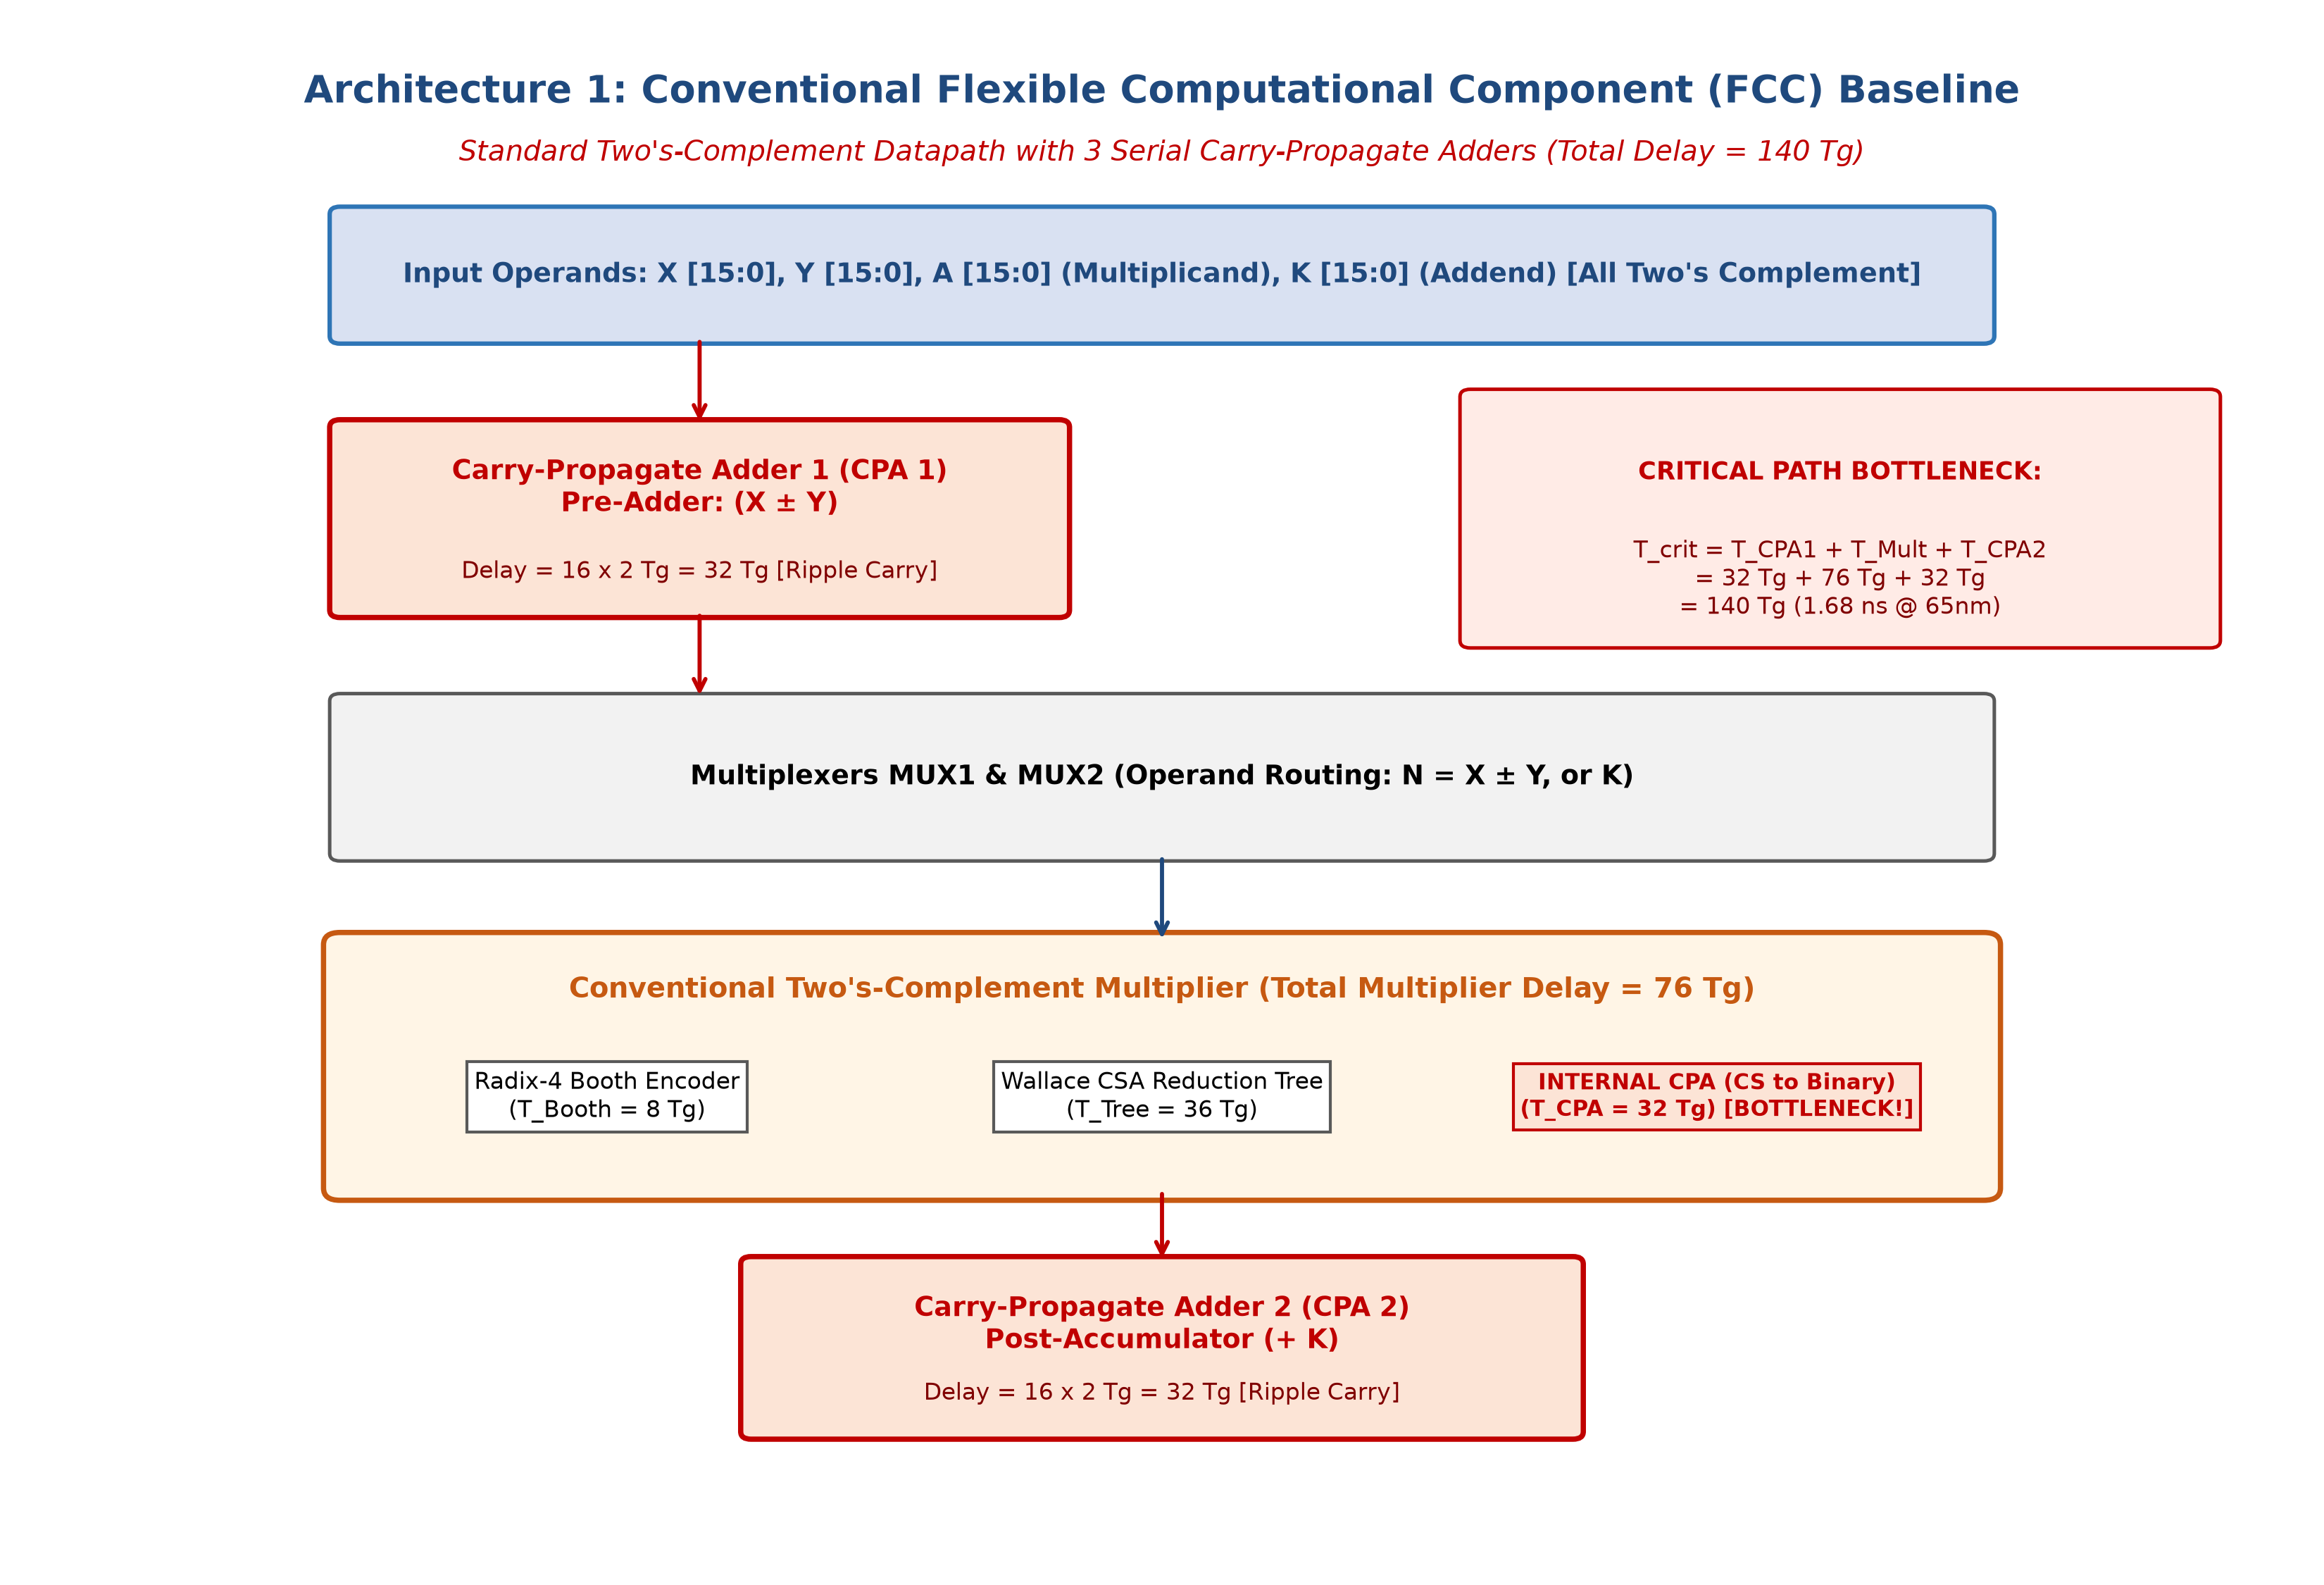
\includegraphics[width=\columnwidth]{figures/arch1_existing_fcc_datapath.png}
\caption{Baseline FCC datapath architecture with three serial carry-propagate adders on the critical path (Total latency: $140\,T_g$).}
\label{fig:arch1}
\end{figure}

Under the Unit Gate Model~\cite{weste2010}, a 16-bit Ripple-Carry CPA contributes $36\,T_g$. The multiplier adds Booth encoding ($8\,T_g$), Wallace reduction ($24\,T_g$), and internal CPA ($36\,T_g$), totaling $68\,T_g$. Along with the post-adder ($36\,T_g$), the total critical path delay is:
\begin{equation}
T_{\text{crit,FCC}} = 36 + 68 + 36 = 140\,T_g \quad (\approx 12.5\text{ ns})
\end{equation}
The FCC occupies $3274\,A_g$, giving an Area-Delay Product of $458,360\,A_g \cdot T_g$.

\section{Proposed Architecture}

\subsection{Top-Level Multi-FCU Accelerator}
The accelerator comprises an array of FCUs connected via a 32-bit dual-rail crossbar interconnect to a dual-ported carry-save scratchpad register file (Fig.~\ref{fig:arch3}). Intermediate values are retained entirely in carry-save form $\{X_C, X_S\}$ and reused without conversion. A single boundary CS-to-Binary CPA is placed strictly at the chip output port.

\begin{figure}[t]
\centering
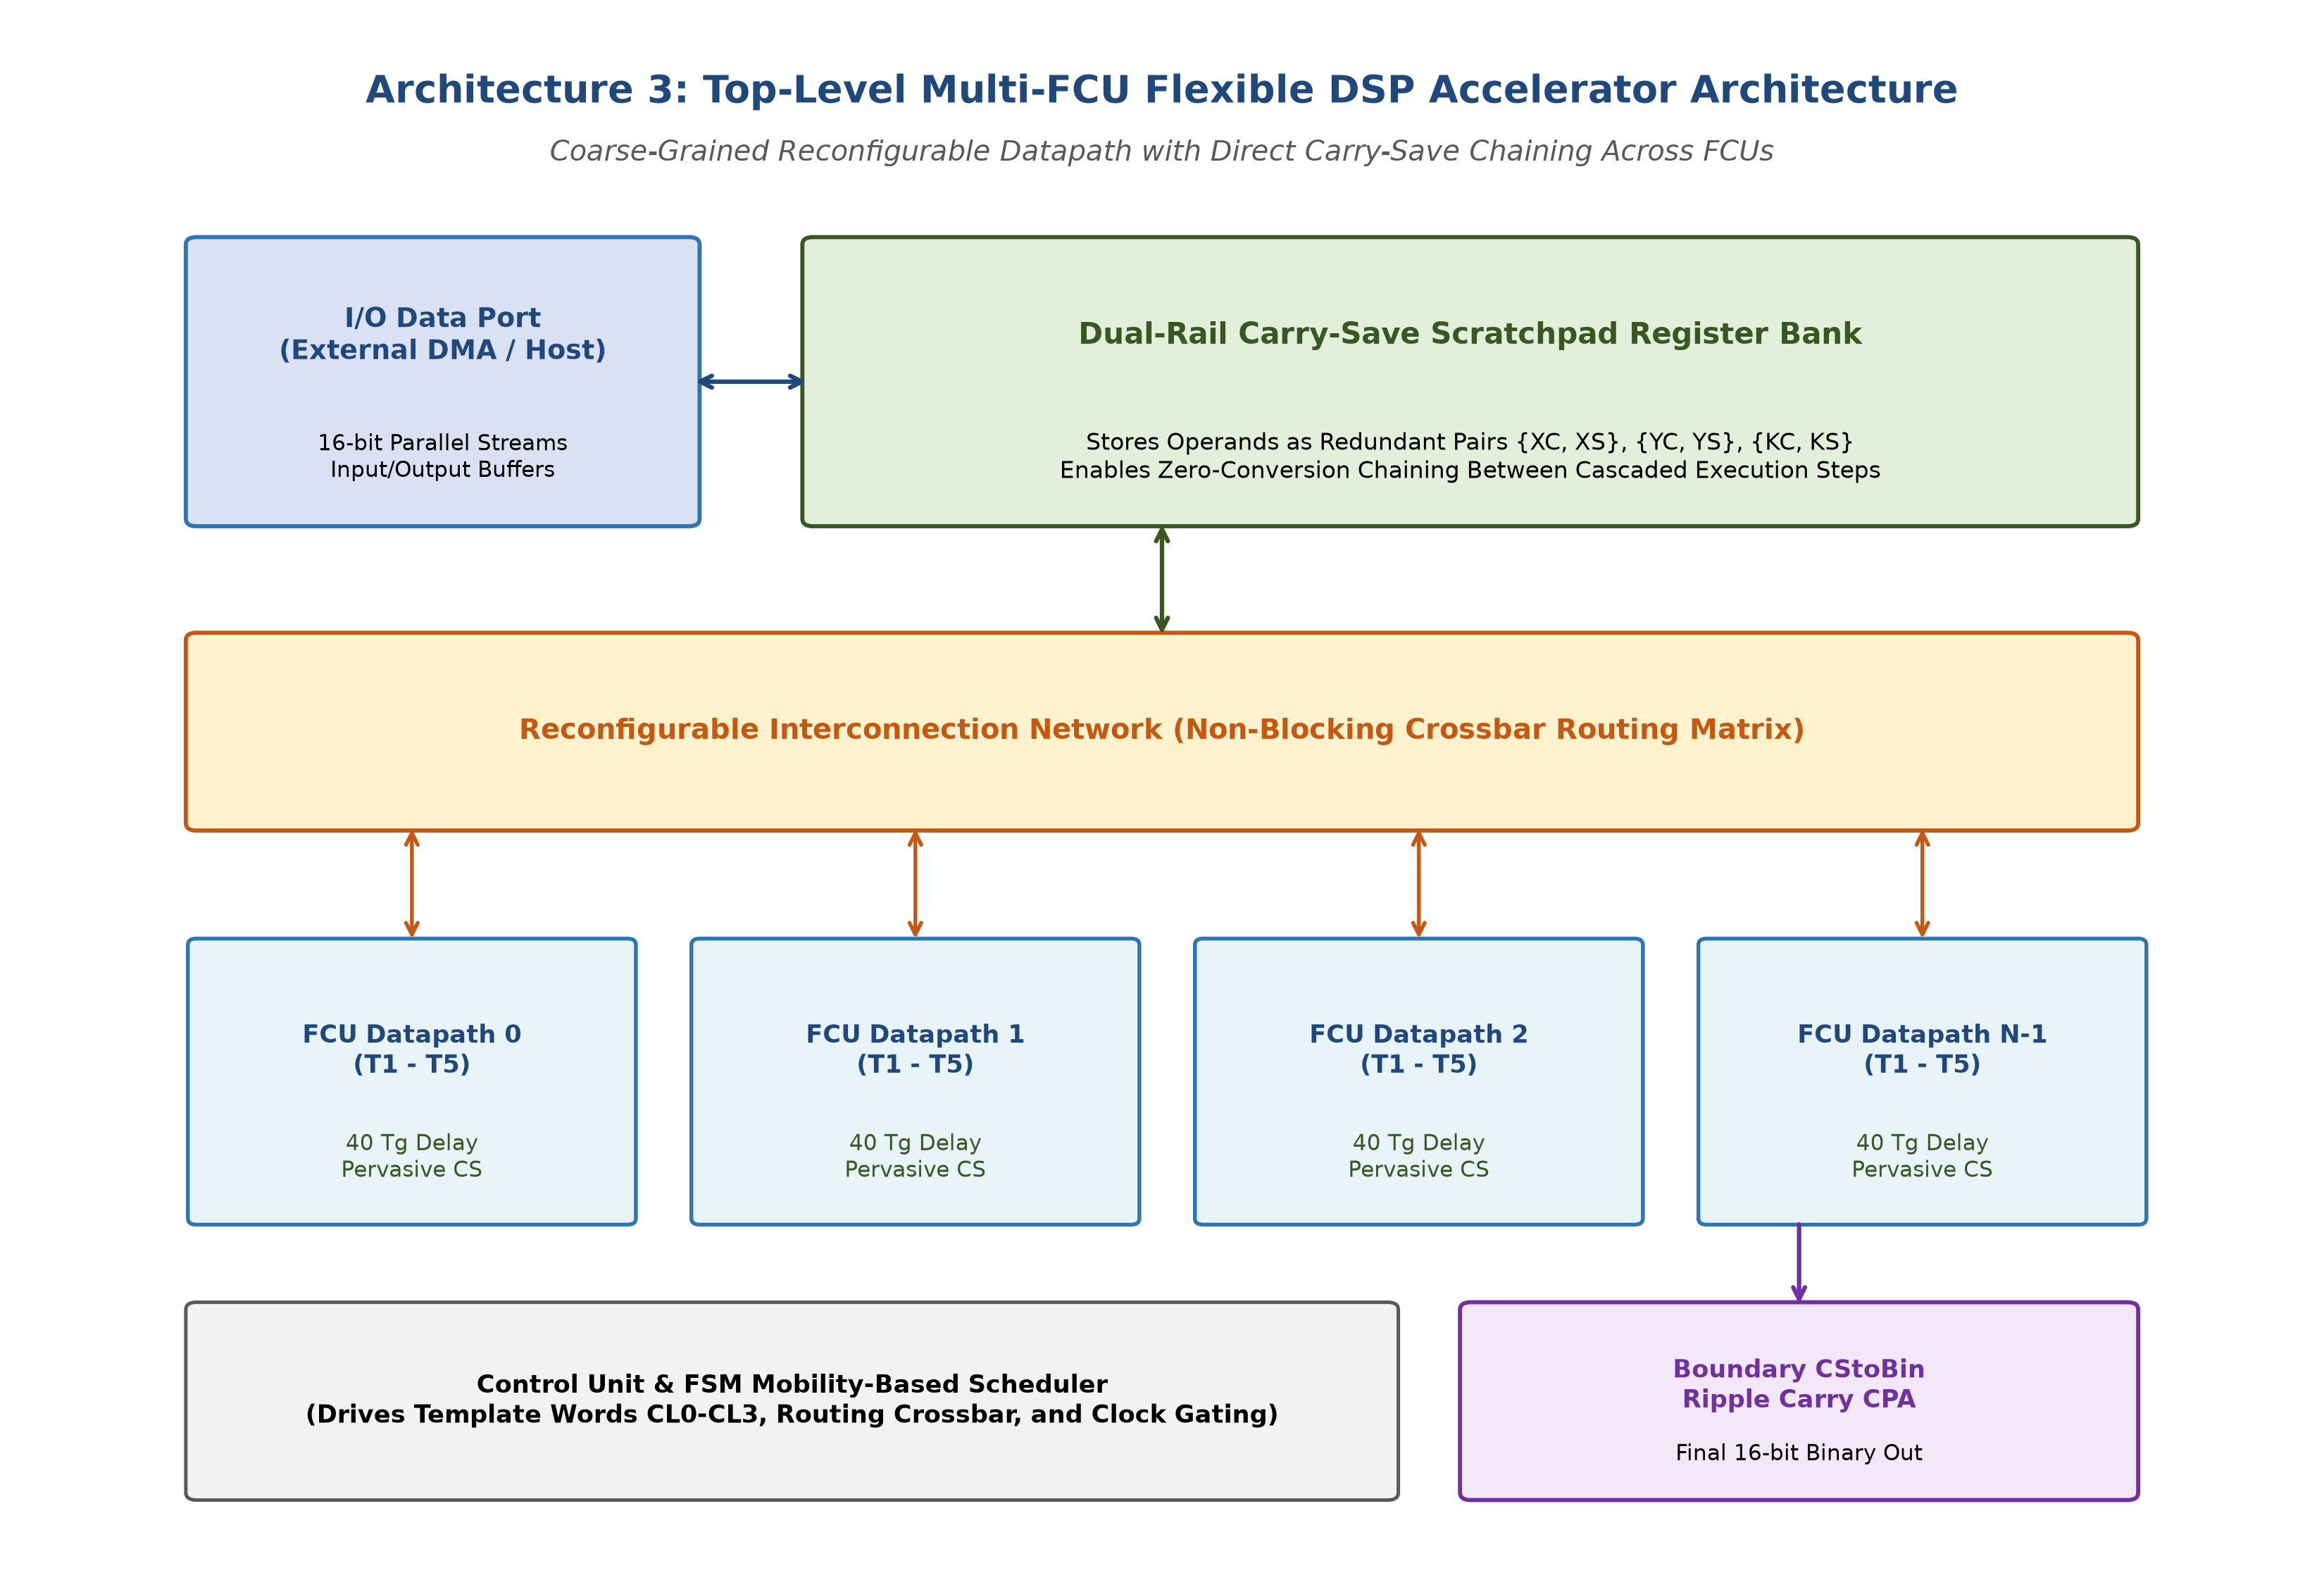
\includegraphics[width=\columnwidth]{figures/arch3_top_level_accelerator_system.png}
\caption{Top-level flexible DSP accelerator architecture with dual-rail scratchpad register bank and crossbar interconnect.}
\label{fig:arch3}
\end{figure}

\subsection{Detailed FCU Microarchitecture}
Each FCU operates on 16-bit redundant carry-save pairs $X^* = \{X_C, X_S\}$ where $X = X_C + X_S$ (Fig.~\ref{fig:arch2}):
\begin{enumerate}
\item \textit{4:2 CS Pre-Compressor}: Computes $X^* \pm Y^*$ in constant $4\,T_g$ delay independent of word length.
\item \textit{Operand Multiplexers (MUX0--MUX3)}: Steer operands dynamically according to \texttt{template\_sel[2:0]}.
\item \textit{Direct CS-to-MB Recoder}: Converts redundant multiplier inputs directly into 8 Radix-4 Booth digits in $8\,T_g$ without intermediate CPA.
\item \textit{3-Level Wallace CSA Multiplier}: Compresses 8 partial products and directly fuses external addends in $12\,T_g$.
\item \textit{Dual-Rail Output Registers}: Captures $W_C$ and $W_S$ via an integrated clock-gating (ICG) cell.
\end{enumerate}

\begin{figure}[t]
\centering
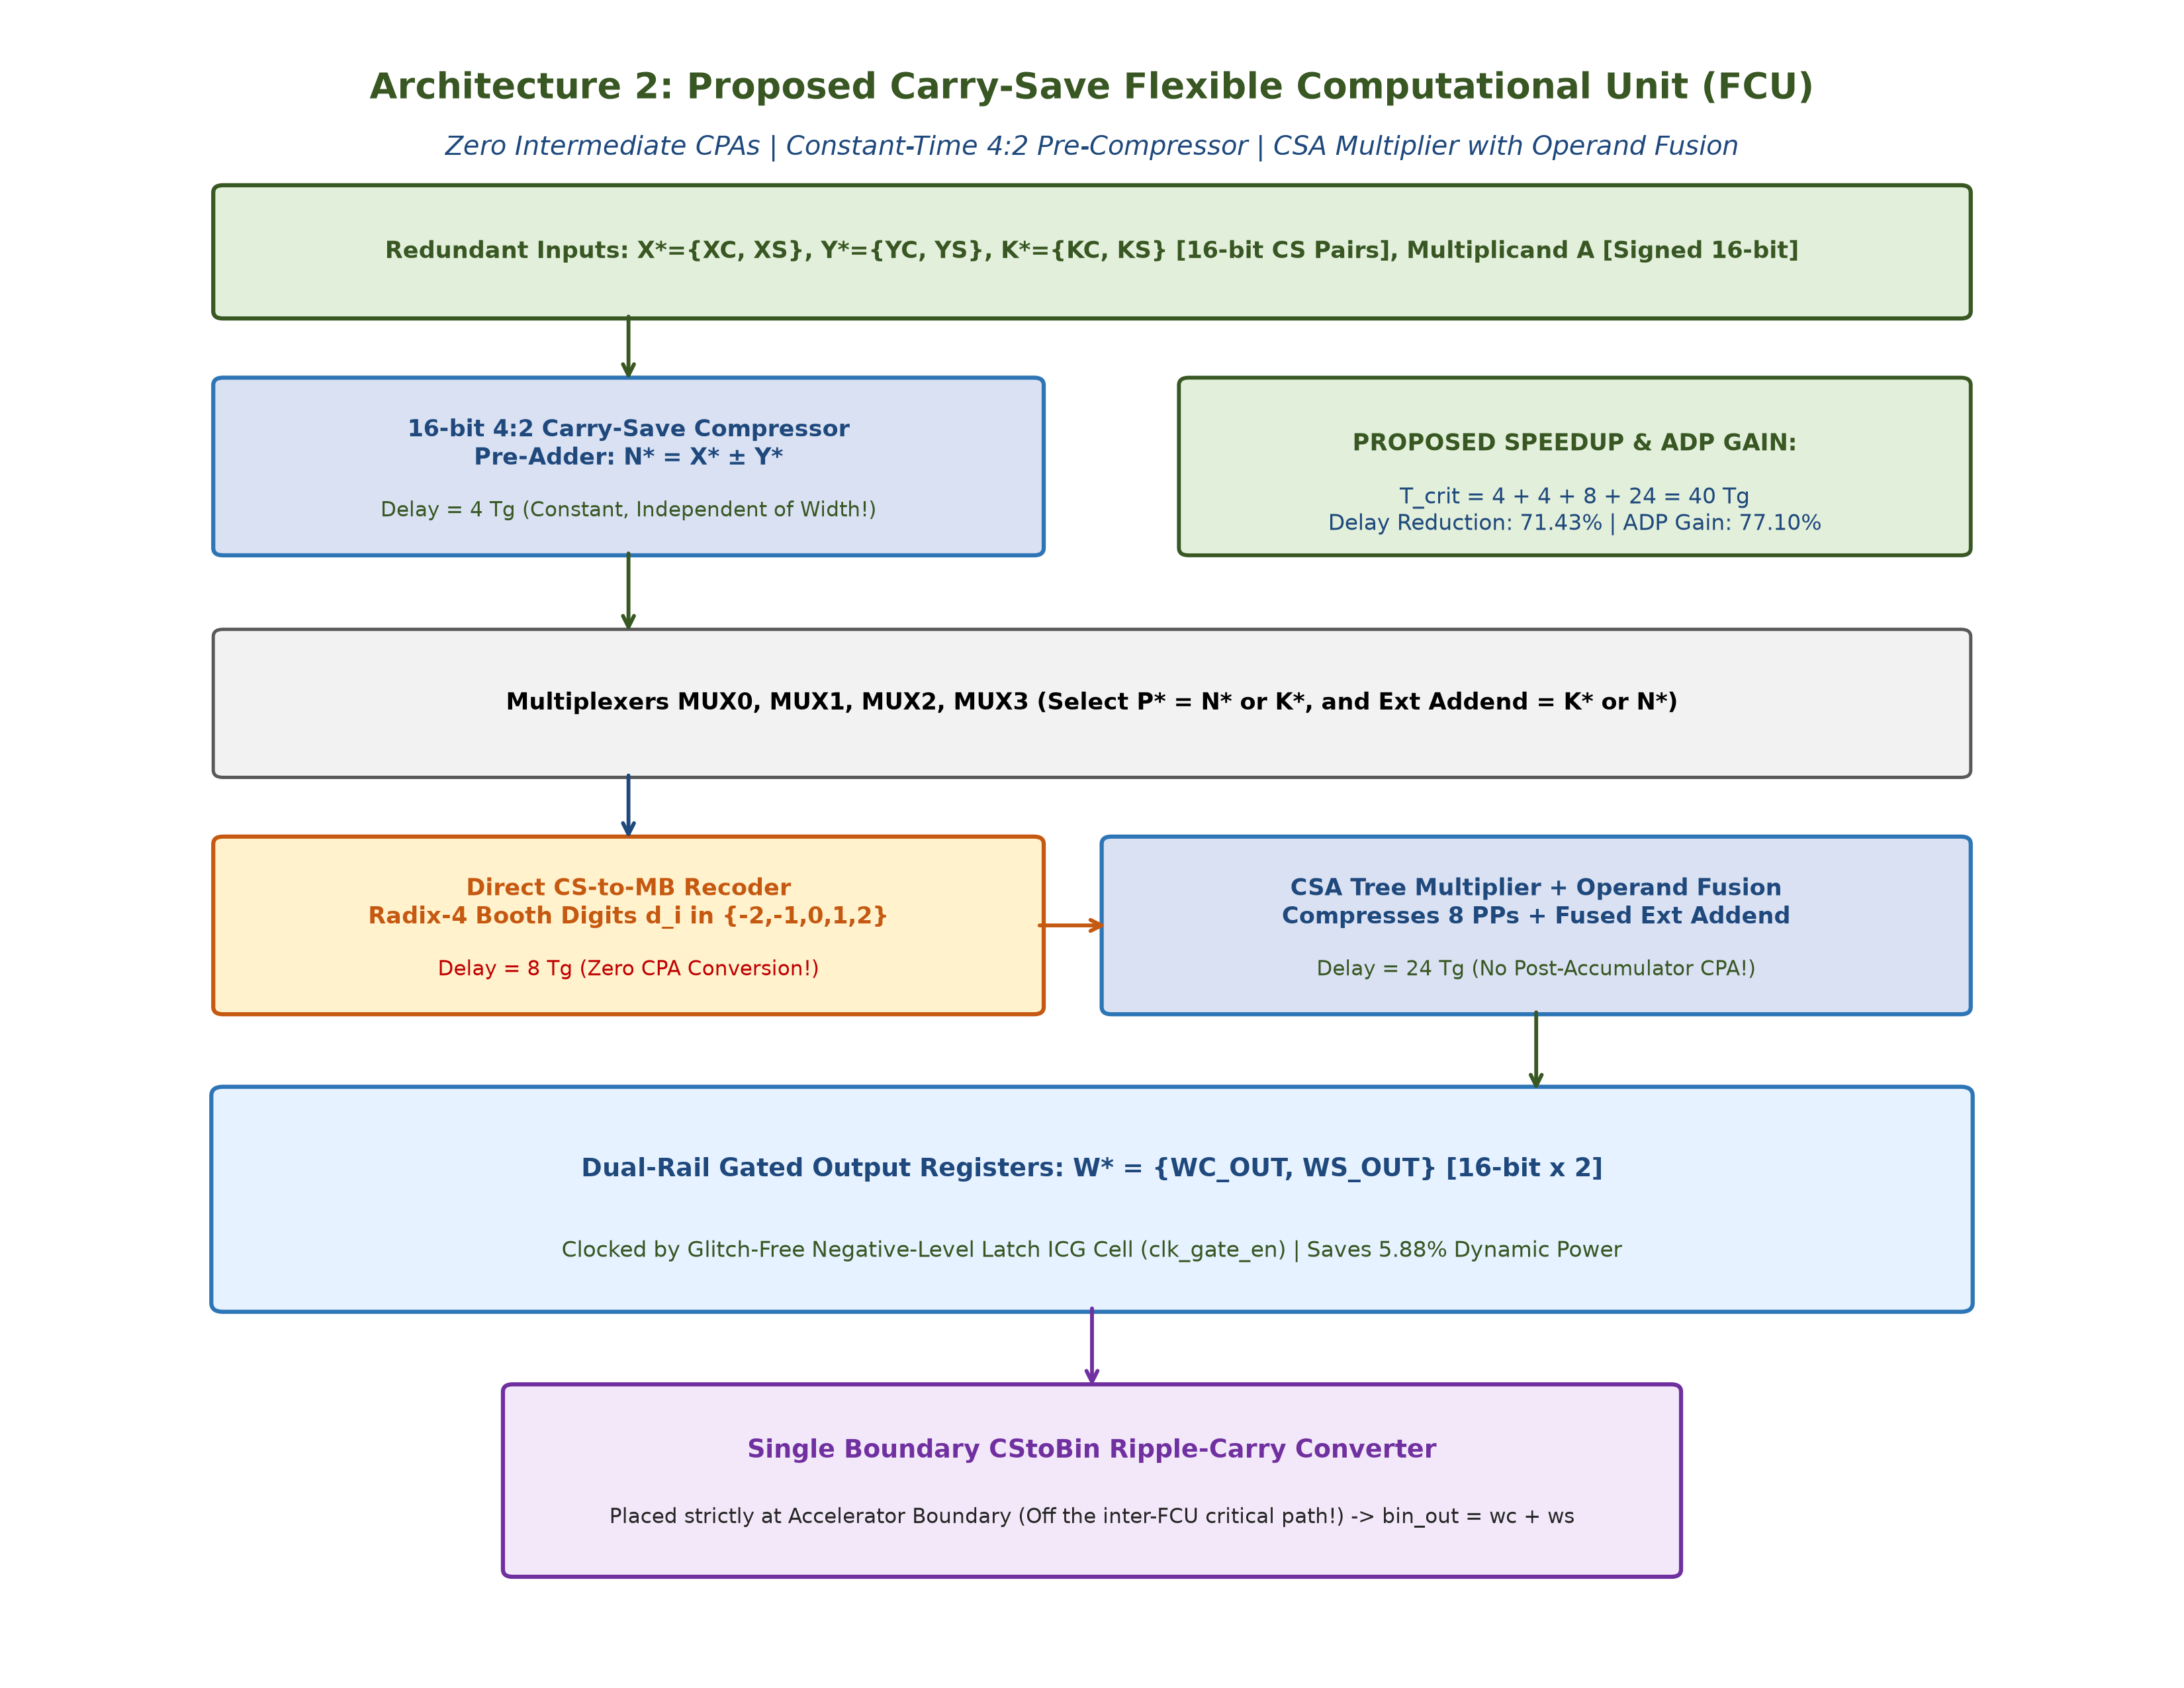
\includegraphics[width=\columnwidth]{figures/arch2_proposed_fcu_microarchitecture.png}
\caption{Microarchitecture of the proposed Carry-Save Flexible Computational Unit (FCU) achieving $40\,T_g$ critical delay.}
\label{fig:arch2}
\end{figure}

\begin{table}[t]
\caption{Supported Operation Templates}
\label{tab:templates}
\centering
\begin{tabular}{lll}
\toprule
\textbf{Template} & \textbf{Function} & \textbf{Target Application} \\
\midrule
\textbf{T1} & $W^* = A \times (X^* + Y^*) + K^*$ & Symmetric FIR Filter / MAC \\
\textbf{T2} & $W^* = A \times (X^* - Y^*) + K^*$ & FFT Radix-2 Butterfly / DCT \\
\textbf{T3} & $W^* = A \times K^* + (X^* + Y^*)$ & Matrix Multiply / Interpolation \\
\textbf{T4} & $W^* = A \times K^* + (X^* - Y^*)$ & Gradient / Motion Estimation \\
\textbf{T5} & $W^* = A \times K^*$ & Direct Coefficient Scaling \\
\bottomrule
\end{tabular}
\end{table}

\begin{figure}[t]
\centering
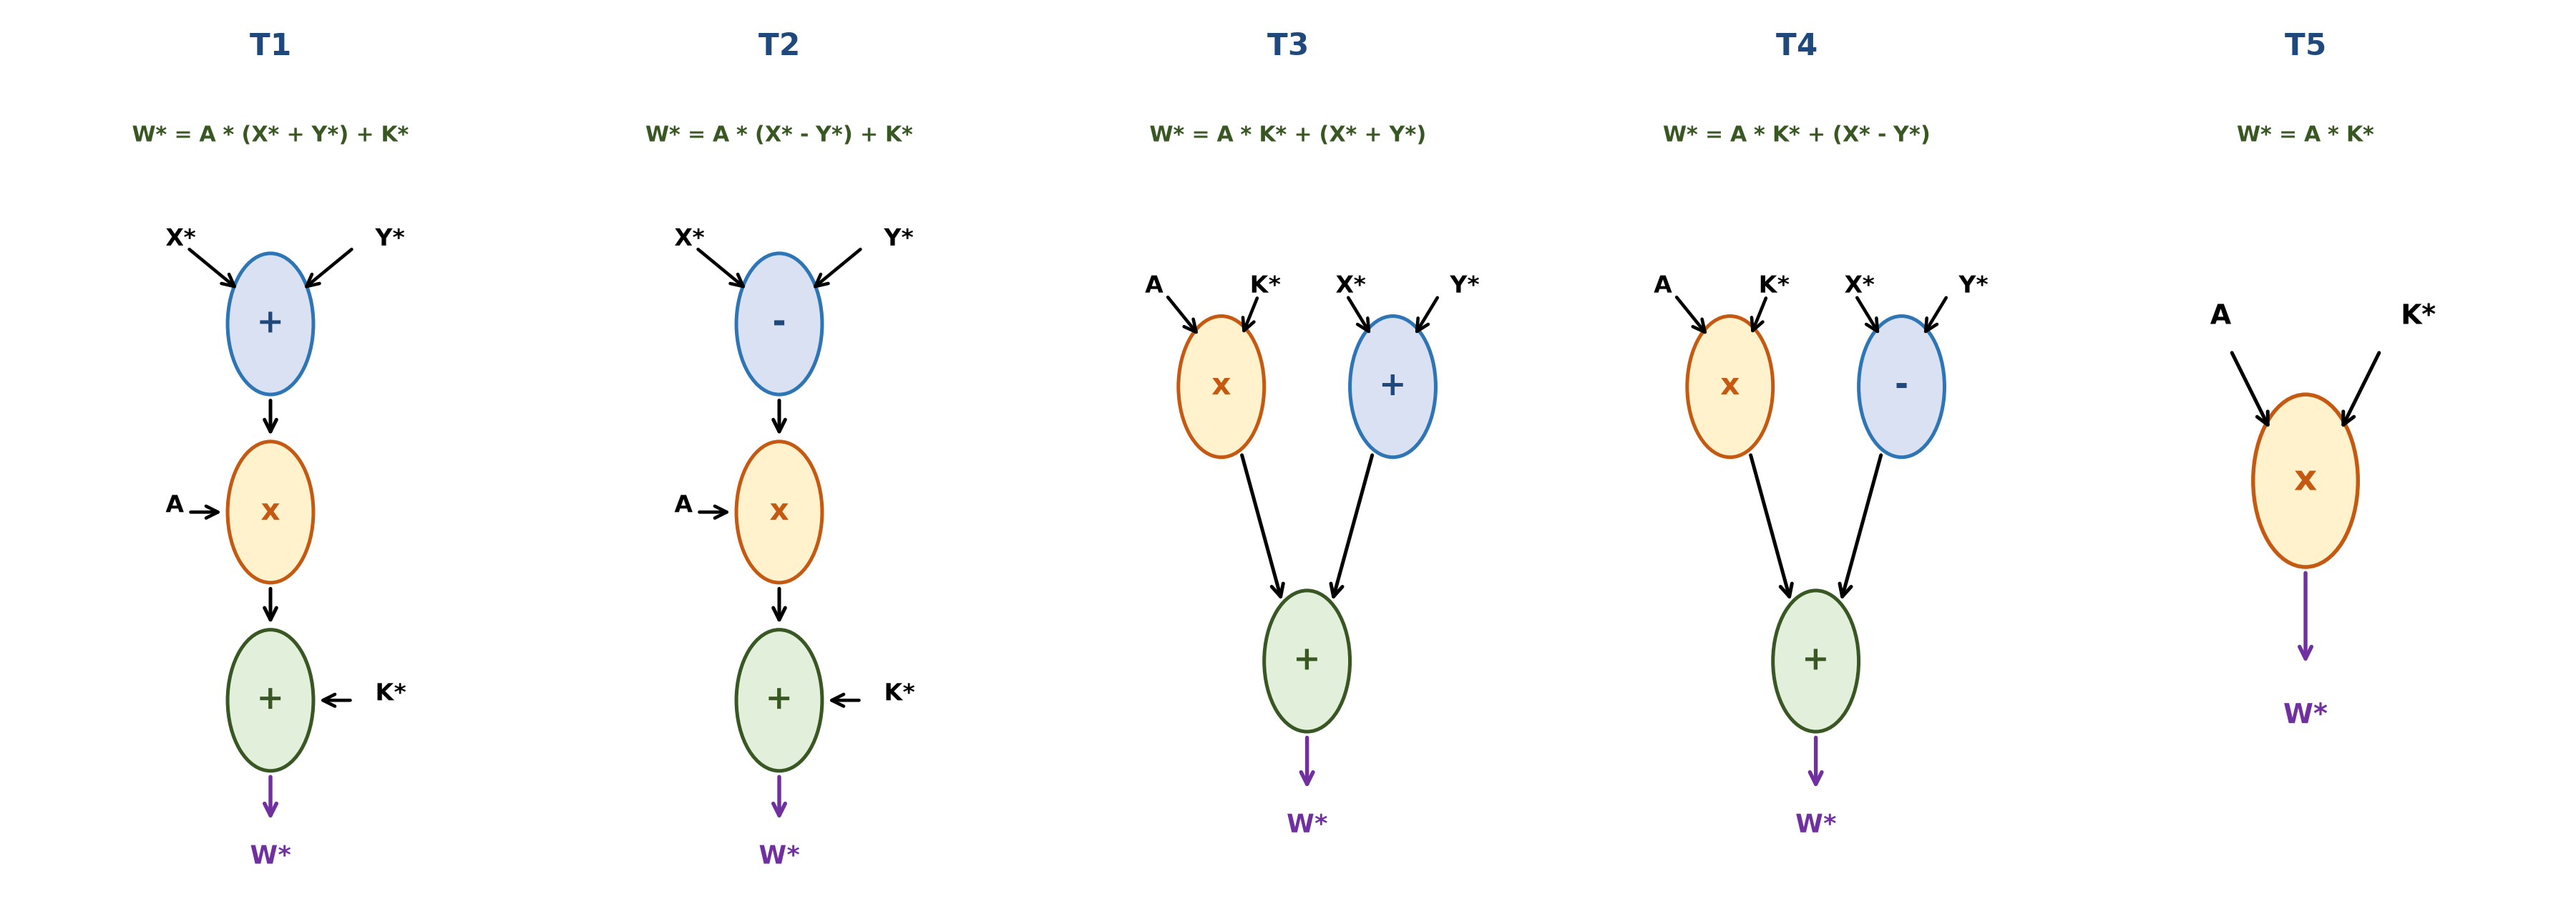
\includegraphics[width=\columnwidth]{figures/arch8_fcu_templates_t1_t5_dataflow.png}
\caption{Data-flow graphs of supported operation templates (T1--T5).}
\label{fig:arch8}
\end{figure}

\section{Design Methodology and Implementation}

\subsection{16-Bit 4:2 Carry-Save Compressor with Subtraction}
The pre-compressor utilizes cascaded Full Adders per bit-slice (Fig.~\ref{fig:arch4}). The horizontal transfer carry $c_{\text{trans}}$ is generated independently of $c_{\text{in}}$:
\begin{equation}
c_{\text{trans}} = (x_1 \land x_2) \lor (x_2 \land x_3) \lor (x_1 \land x_3)
\end{equation}
For subtraction ($X^* - Y^*$), $Y_C$ and $Y_S$ are inverted bitwise and two $+1$ carry-ins are injected via \texttt{cin1=1} and \texttt{cin2=1}, achieving subtraction with the exact same $4\,T_g$ delay as addition.

\begin{figure}[t]
\centering
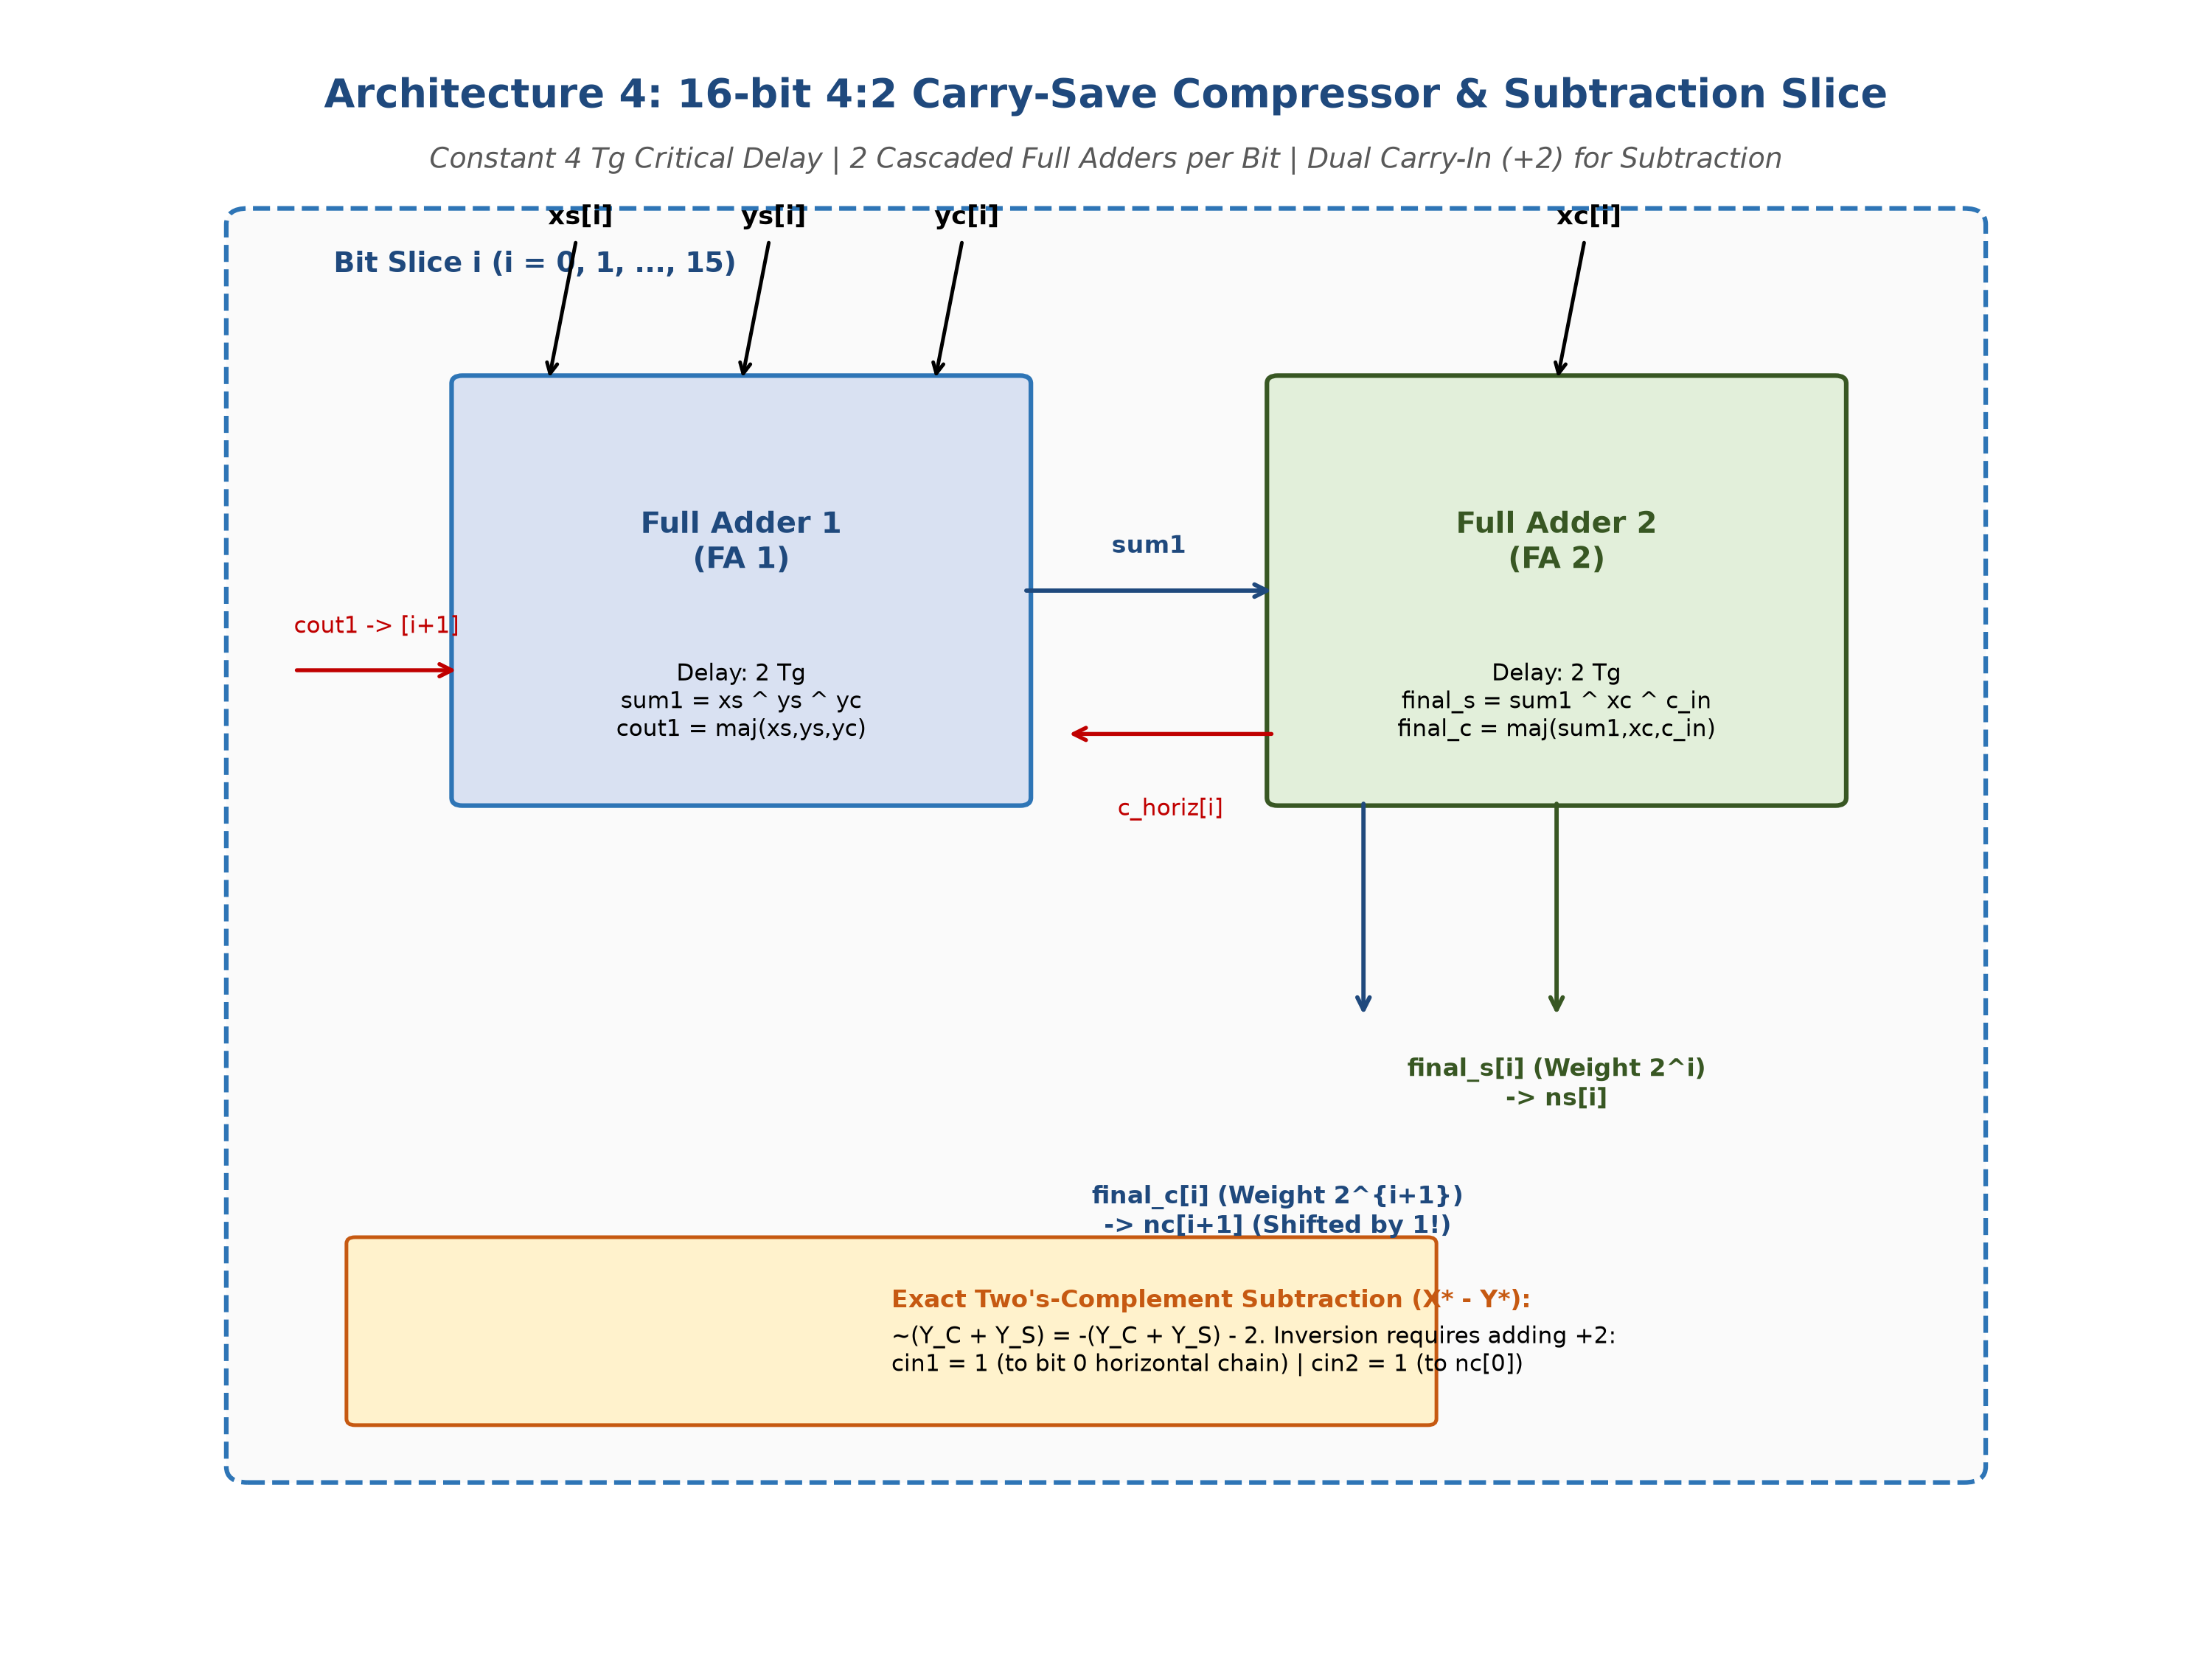
\includegraphics[width=\columnwidth]{figures/arch4_compressor_4_2_slice.png}
\caption{Gate-level bit-slice schematic of the 16-bit 4:2 Carry-Save Compressor with dual carry-in subtraction support ($4\,T_g$ delay).}
\label{fig:arch4}
\end{figure}

\subsection{Direct CS-to-Modified Booth Recoder}
The recoder converts $\{C, S\}$ directly into 8 Radix-4 digits $d_j \in \{-2, -1, 0, +1, +2\}$ in three stages without a carry-propagate adder (Fig.~\ref{fig:arch5}). Carry transfers $t_j$ are strictly bounded within adjacent 2-bit windows, achieving full recoding in $8\,T_g$.

\begin{figure}[t]
\centering
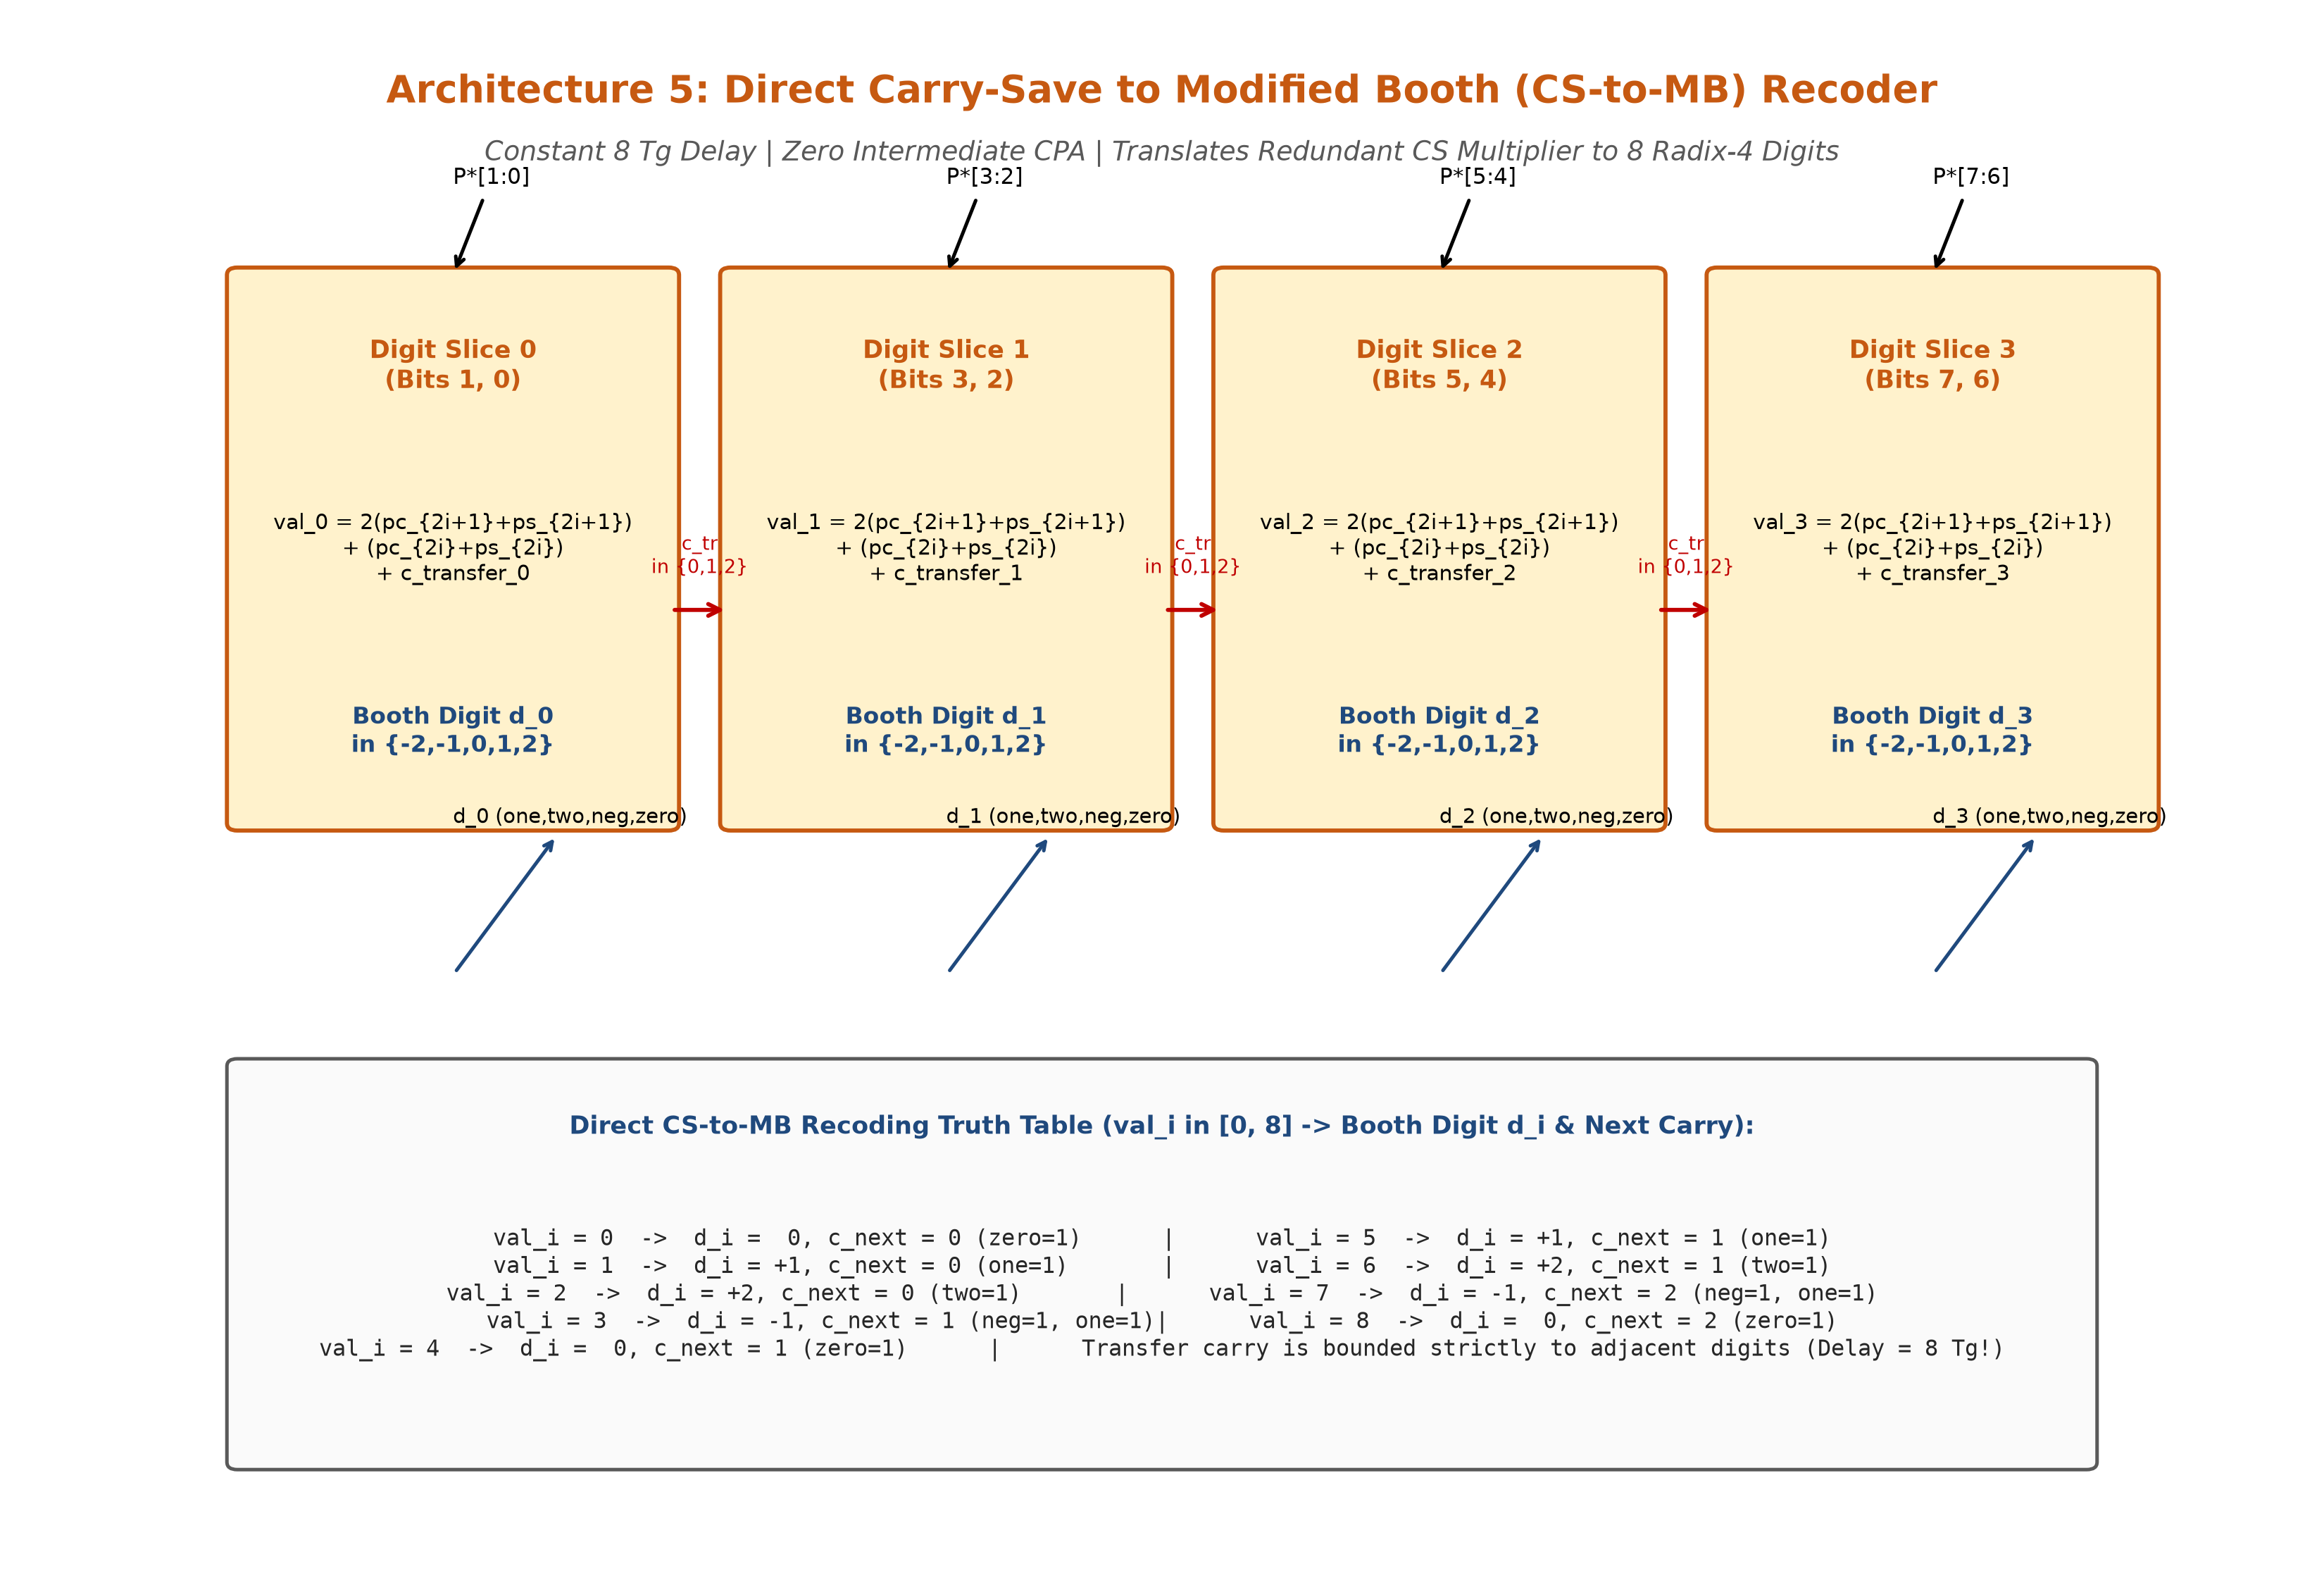
\includegraphics[width=\columnwidth]{figures/arch5_cs_to_mb_recoder_stages.png}
\caption{Direct CS-to-Modified Booth (CS-to-MB) recoder architecture showing 3-stage localized carry transfer.}
\label{fig:arch5}
\end{figure}

\subsection{3-Level Wallace CSA Multiplier Reduction Tree}
As illustrated in Fig.~\ref{fig:arch6}, the multiplier core reduces 8 partial products (PP0--PP7) and fuses external addends ($ext\_c, ext\_s$) across three 4:2 compressor levels:
\begin{itemize}
\item \textit{Level 1}: Compresses PP0--PP7 to 4 intermediate vectors ($4\,T_g$).
\item \textit{Level 2}: Compresses 4 vectors to 2 pure product vectors ($4\,T_g$).
\item \textit{Level 3 (Fusion)}: Compresses product vectors directly with $ext\_c$ and $ext\_s$ to form $W_C$ and $W_S$ ($4\,T_g$).
\end{itemize}
Total reduction tree latency is $12\,T_g$ with zero intermediate CPA.

\begin{figure}[t]
\centering
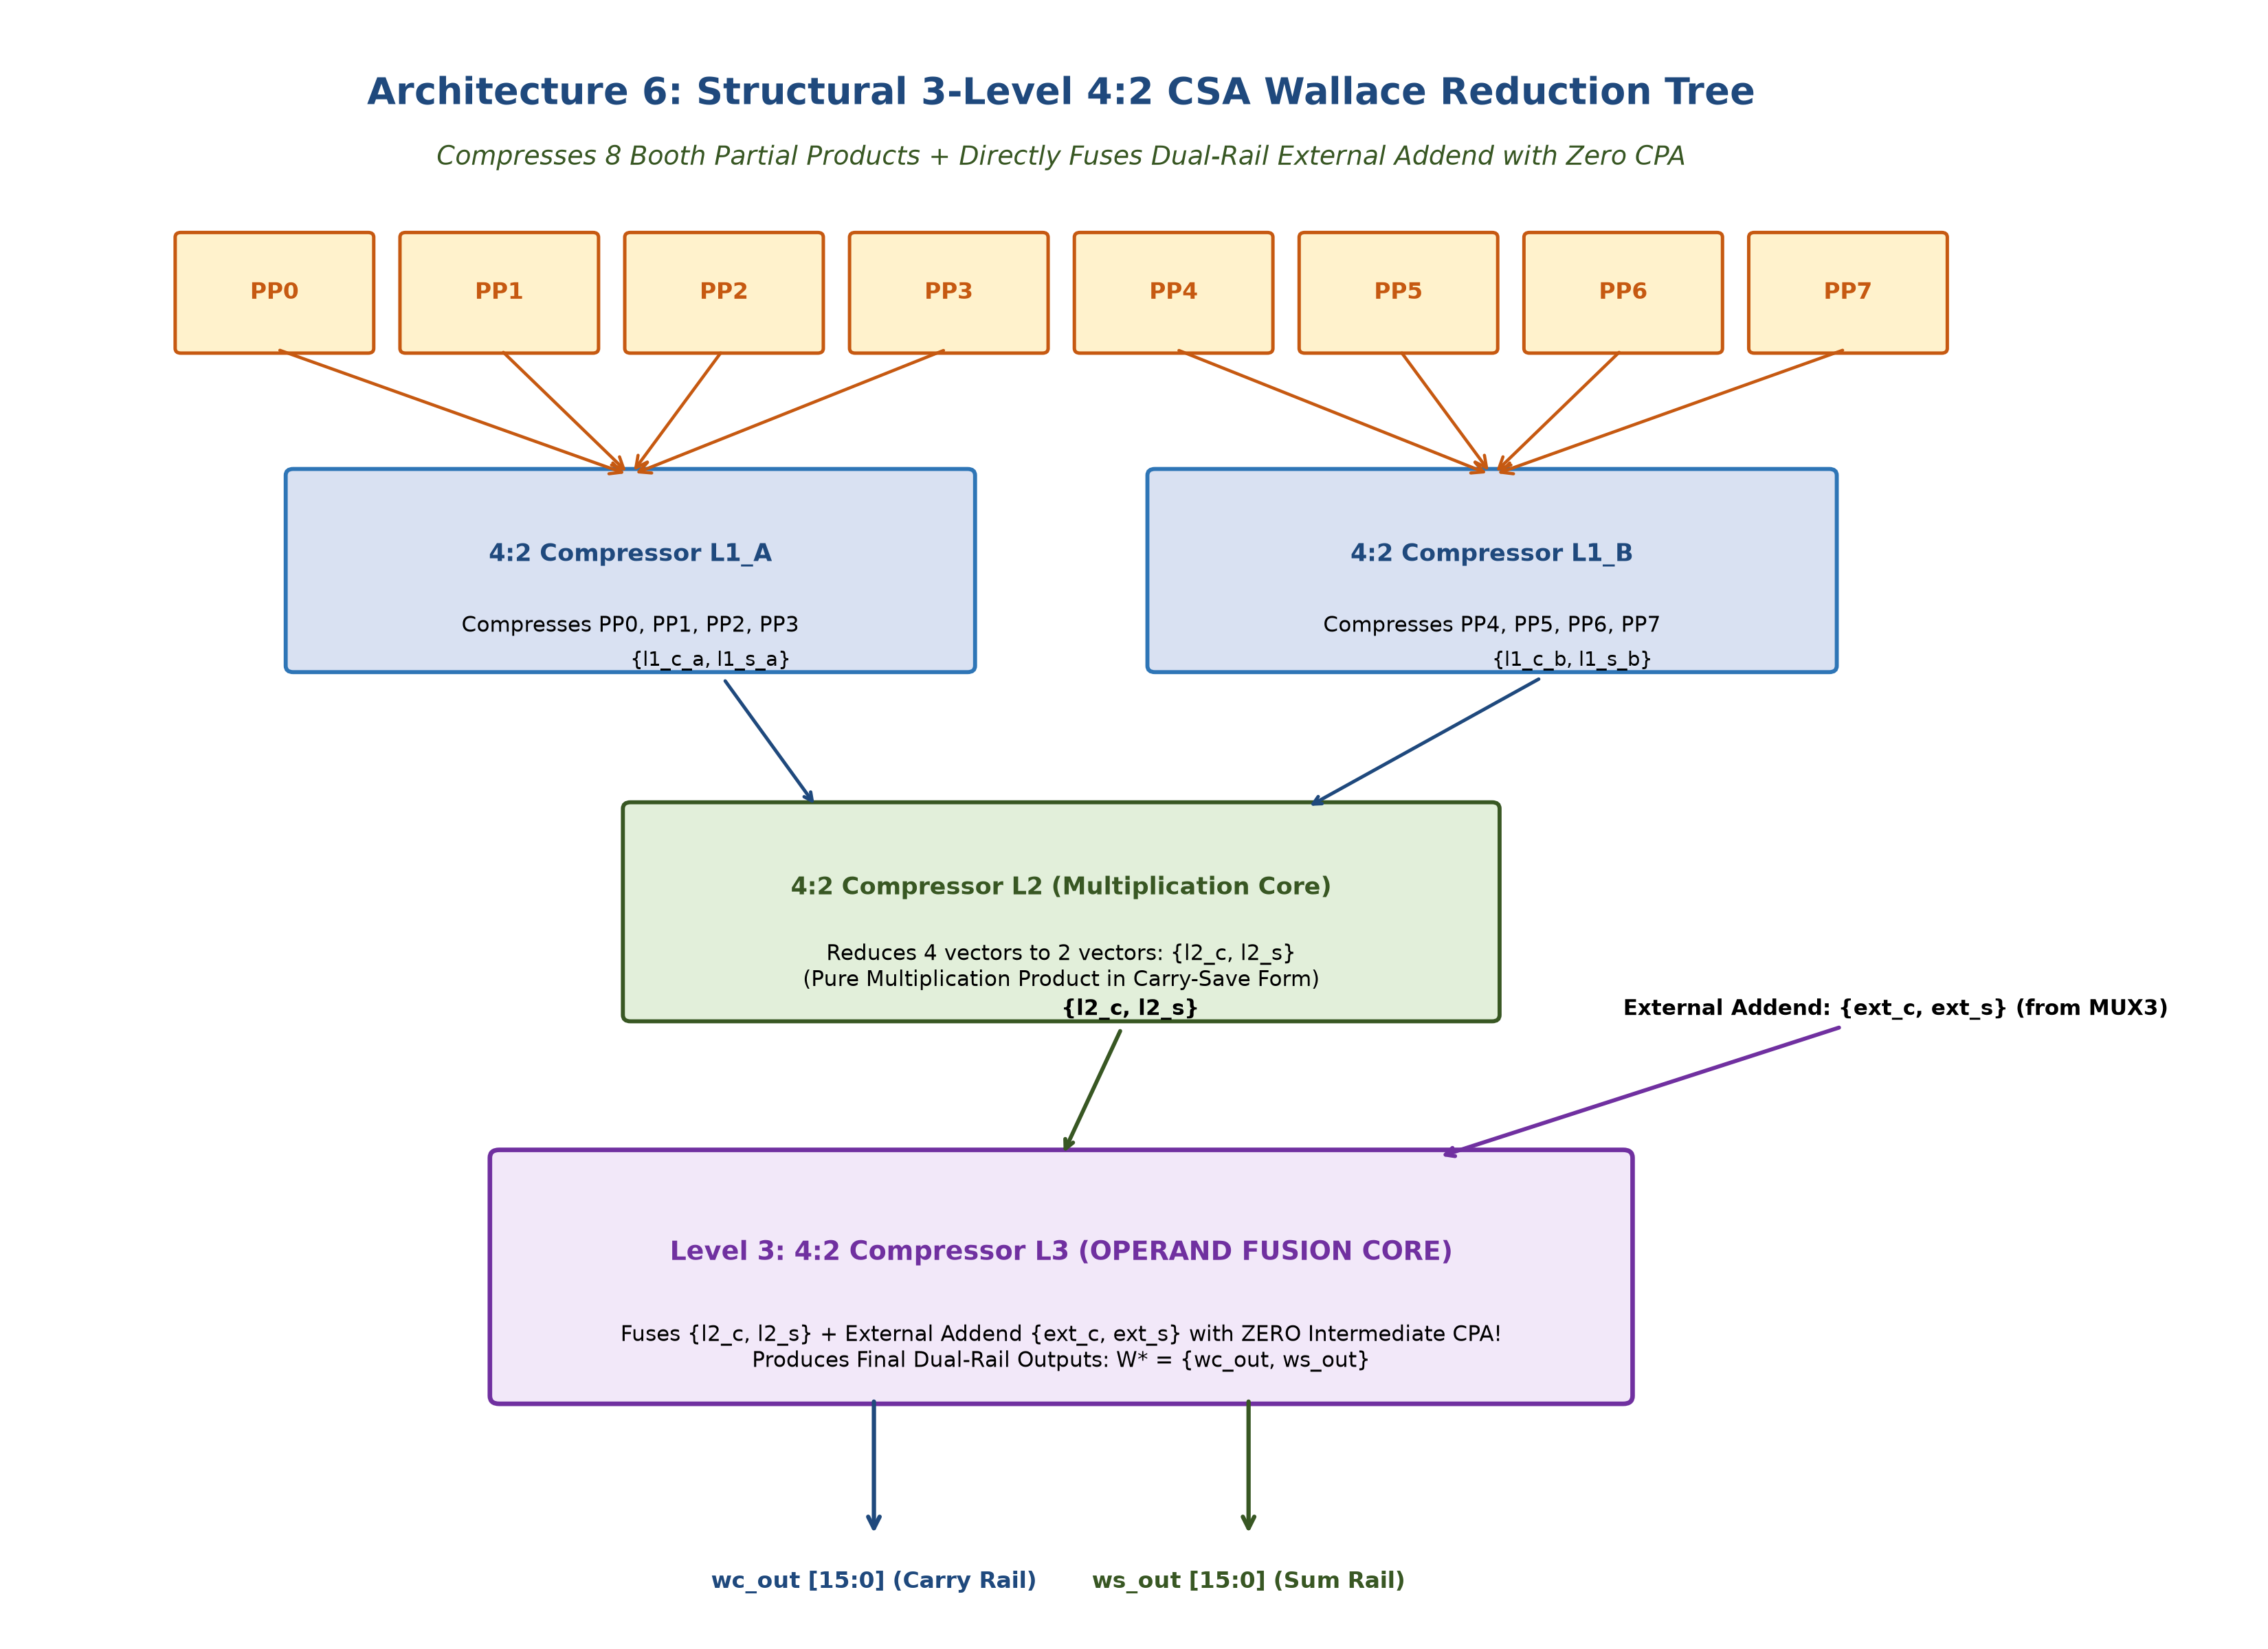
\includegraphics[width=\columnwidth]{figures/arch6_csa_multiplier_tree_reduction.png}
\caption{Structural 3-Level 4:2 Wallace CSA multiplier reduction tree with direct external operand fusion.}
\label{fig:arch6}
\end{figure}

\subsection{Dual-Rail Integrated Clock Gating (ICG)}
To eliminate dynamic power during idle cycles without introducing rail skew, an active-low latch ICG cell gates the master clock for both $W_C$ and $W_S$ register banks simultaneously (Fig.~\ref{fig:arch7}):
\begin{equation}
\text{gclk} = \text{clk} \land Q_{\text{latch}}
\end{equation}

\begin{figure}[t]
\centering
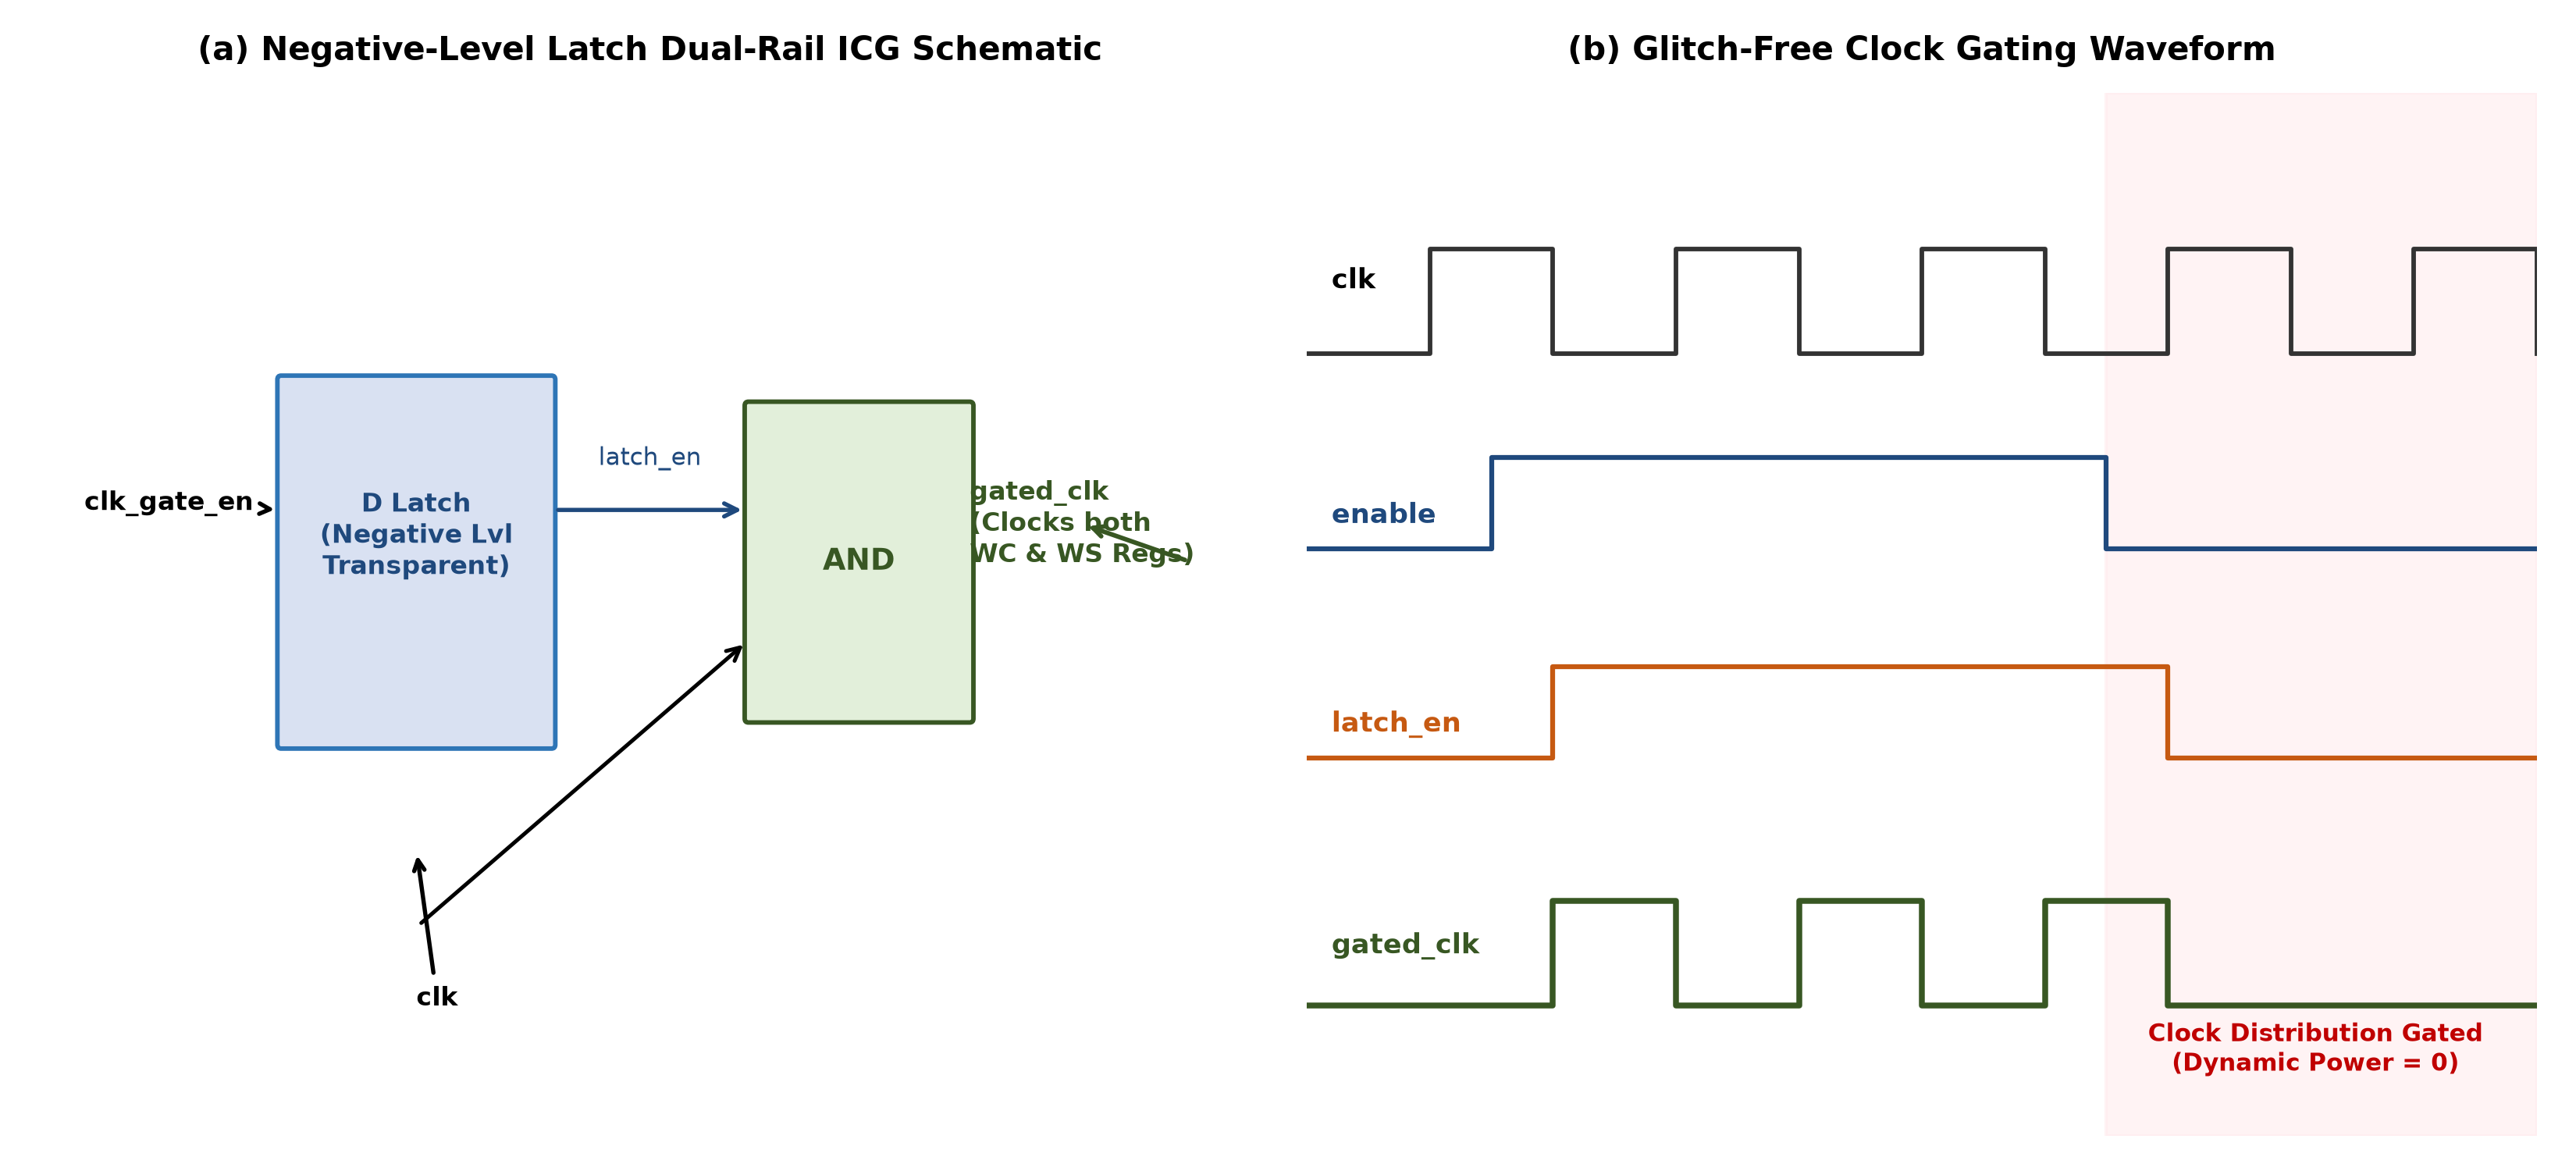
\includegraphics[width=\columnwidth]{figures/arch7_dual_rail_icg_clock_gating.png}
\caption{Dual-Rail Integrated Clock Gating (ICG) schematic and glitch-free timing waveform.}
\label{fig:arch7}
\end{figure}

\section{Simulation and Functional Verification}
The proposed design was implemented in synthesizable Verilog RTL and exhaustively verified in Xilinx Vivado XSim. A complete 112-vector testbench verified directed templates, negative operands, zero corners, and 100 randomized trials with zero functional errors (\texttt{errors = 00000000}).

\begin{table}[t]
\caption{Functional Verification Results (112 Vectors)}
\label{tab:verification}
\centering
\begin{tabular}{lcl}
\toprule
\textbf{Test Section} & \textbf{Count} & \textbf{Verification Target} \\
\midrule
Directed Positives & 5 & Verified T1--T5 nominal values \\
Signed Operands & 3 & Two's-complement negative inputs \\
Corner Boundaries & 2 & Zero multiplicand \& multiplier \\
Dual-Rail ICG & 2 & Output held flat across 4 gated cycles \\
Randomized Trials & 100 & Equivalence against mathematical model \\
\midrule
\textbf{Total} & \textbf{112} & \textbf{100\% ALL PASSED (Zero errors)} \\
\bottomrule
\end{tabular}
\end{table}

\section{Performance Analysis and Comparison}

\subsection{Hardware Complexity and Critical-Path Delay}
Under the Unit Gate Model, the proposed FCU critical path delay is:
\begin{equation}
T_{\text{crit,FCU}} = 4 + 8 + 12 + 16 = 40\,T_g
\end{equation}
Compared to $140\,T_g$ for the baseline FCC, this represents a \textbf{71.43\% latency reduction ($3.5\times$ speedup)}. Gate-equivalent area decreases by \textbf{19.85\%} ($3274\,A_g \to 2624\,A_g$), yielding a \textbf{77.10\% improvement in Area-Delay Product (ADP)}.

\begin{table}[t]
\caption{Hardware Metric Comparison (Theoretical Model)}
\label{tab:hardware}
\centering
\begin{tabular}{lccc}
\toprule
\textbf{Metric} & \textbf{Existing FCC}~\cite{galanis2006} & \textbf{Proposed FCU} & \textbf{Gain} \\
\midrule
Intermediate CPAs & 3 CPAs & \textbf{0 CPAs} & Eliminated \\
Critical Path ($T_g$) & $140.0\,T_g$ & $\mathbf{40.0\,T_g}$ & \textbf{71.43\%} \\
Est. Delay @ 65 nm & 1.68 ns & \textbf{1.13 ns} & 32.74\% \\
Gate Area ($A_g$) & $3274.0\,A_g$ & $\mathbf{2624.0\,A_g}$ & \textbf{19.85\%} \\
ADP ($A_g \cdot T_g$) & 458,360 & \textbf{104,960} & \textbf{77.10\%} \\
\bottomrule
\end{tabular}
\end{table}

\begin{figure}[t]
\centering
\includegraphics[width=\columnwidth]{figures/chart19_area_comparison.png}
\caption{Gate-equivalent area and Area-Delay Product (ADP) comparison between FCC and proposed FCU.}
\label{fig:chart19}
\end{figure}

\begin{figure}[t]
\centering
\includegraphics[width=\columnwidth]{figures/chart20_delay_comparison.png}
\caption{Critical-path delay stacked stage breakdown: $140\,T_g$ (FCC) vs $40\,T_g$ (Proposed FCU).}
\label{fig:chart20}
\end{figure}

\subsection{Kernel Energy Benchmark Results}
Three DSP benchmark kernels were mapped onto both datapaths. As shown in Fig.~\ref{fig:chart21}, the proposed FCU achieves substantial energy reductions: \textbf{31.42\% for FIR16} (1038.0 $\to$ 711.9~pJ), \textbf{38.57\% for Elliptic} (261.0 $\to$ 160.4~pJ), and \textbf{41.24\% for Volterra} (391.3 $\to$ 229.9~pJ), averaging a 37.08\% overall energy reduction.

\begin{figure}[t]
\centering
\includegraphics[width=\columnwidth]{figures/chart21_energy_comparison.png}
\caption{DSP benchmark kernel energy consumption comparison (FIR16, Elliptic, and Volterra filters).}
\label{fig:chart21}
\end{figure}

\subsection{Physical FPGA Synthesis Results (Vivado 2022.2)}
The design was synthesized on a Xilinx Artix-7 FPGA (\texttt{xc7a200tfbg676-2}) under a 100~MHz clock constraint (10.000~ns period). The synthesis report confirms an ultra-compact footprint: \textbf{368 LUTs (0.27\%)} and \textbf{31 Flip-Flops (0.01\%)} with positive slack ($\text{WNS} > 0$, $\text{TNS} = 0.000\text{ ns}$), verifying physical realizability.

\section{Conclusion}
This paper presented an energy-efficient Flexible Computational Unit (FCU) for DSP accelerators. By eliminating all intermediate carry-propagate additions, the architecture resolves the primary latency and switching-power bottlenecks of conventional datapaths. The FCU achieves a 71.43\% latency reduction ($3.5\times$ speedup), a 19.85\% area reduction, a 77.10\% ADP improvement, and up to 41.24\% kernel energy savings. Physical FPGA synthesis on a Xilinx Artix-7 device validates hardware efficiency with only 368 LUTs and full 100~MHz timing closure.

\begin{thebibliography}{00}
\bibitem{tsoumanis2016} K. Tsoumanis, S. Xydis, G. Zervakis, and K. Pekmestzi, ``Flexible DSP accelerator architecture exploiting carry-save arithmetic,'' \textit{IEEE Trans. Very Large Scale Integr. (VLSI) Syst.}, vol. 24, no. 1, pp. 368--372, Jan. 2016.
\bibitem{galanis2006} M. D. Galanis, G. Theodoridis, S. Tragoudas, and C. E. Goutis, ``A high-performance data path for synthesizing DSP kernels,'' \textit{IEEE Trans. Comput.-Aided Design Integr. Circuits Syst.}, vol. 25, no. 6, pp. 1154--1162, Jun. 2006.
\bibitem{xydis2011} S. Xydis, G. Economakos, D. Soudris, and K. Pekmestzi, ``High performance and area efficient flexible DSP datapath synthesis,'' \textit{IEEE Trans. VLSI Syst.}, vol. 19, no. 3, pp. 429--442, Mar. 2011.
\bibitem{kim2000} T. Kim and J. Um, ``A practical approach to the synthesis of arithmetic circuits using carry-save-adders,'' \textit{IEEE Trans. Comput.-Aided Design Integr. Circuits Syst.}, vol. 19, no. 5, pp. 615--624, May 2000.
\bibitem{verma2008} A. K. Verma, P. Brisk, and P. Ienne, ``Data-flow transformations to maximize the use of carry-save representation in arithmetic circuits,'' \textit{IEEE Trans. Comput.-Aided Design Integr. Circuits Syst.}, vol. 27, no. 10, pp. 1761--1774, Oct. 2008.
\bibitem{tsoumanis2014} K. Tsoumanis, S. Xydis, C. Efstathiou, N. Moschopoulos, and K. Pekmestzi, ``An optimized modified Booth recoder for efficient design of the add-multiply operator,'' \textit{IEEE Trans. Circuits Syst. I, Reg. Papers}, vol. 61, no. 4, pp. 1133--1143, Apr. 2014.
\bibitem{parhami2010} B. Parhami, \textit{Computer Arithmetic: Algorithms and Hardware Designs}, 2nd ed. Oxford, U.K.: Oxford Univ. Press, 2010.
\bibitem{weste2010} N. H. E. Weste and D. M. Harris, \textit{CMOS VLSI Design: A Circuits and Systems Perspective}, 4th ed. Boston, MA: Addison-Wesley, 2010.
\bibitem{ansaloni2011} G. Ansaloni, P. Bonzini, and L. Pozzi, ``EGRA: A coarse grained reconfigurable architectural template,'' \textit{IEEE Trans. VLSI Syst.}, vol. 19, no. 6, pp. 1062--1074, Jun. 2011.
\end{thebibliography}

\end{document}

